% Параграф №2 из труда Эйлера "Новая теория движения Луны" (Эйлер Л. Новая
% теория движения Луны. Перевод с латинского акад. А. Н. Крылова. М.-Л.:
% изд-во АН СССР, 1937. 248 с.).
% Задание выполнено в ходе ознакомления с курсом "Документы и презентации % в LaTex", разработанным Данилом Фёдоровых (danil@fedorovykh.ru),
% записанном НИУ ВШЭ
% для Coursera.org: http://coursera.org/course/latex .

\documentclass[a4paper,12pt]{article} % добавить leqno в [] для нумерации слева


%%% Работа с русским языком
\usepackage{cmap}					% поиск в PDF
\usepackage{mathtext} 				% русские буквы в фомулах
\usepackage[T2A]{fontenc}			% кодировка
\usepackage[utf8]{inputenc}			% кодировка исходного текста
\usepackage[english,russian]{babel}	% локализация и переносы


%%% Работа с картинками
\usepackage{graphicx}  % Для вставки рисунков
\graphicspath{{images/}{images2/}}  % папки с картинками
\setlength\fboxsep{3pt} % Отступ рамки \fbox{} от рисунка
\setlength\fboxrule{1pt} % Толщина линий рамки \fbox{}
\usepackage{wrapfig} % Обтекание рисунков и таблиц текстом

\usepackage {caption}
\usepackage {textcomp}
\usepackage {floatrow}
%\floatsetup[figure]{capposition=bottom, floatwidth=0.9\linewidth, margins=centering}

	
	
% Первая из этих строк запретит все разрывы строк после знаков
% бинарных операций, а вторая — после знаков бинарных отношений, и
% при этом помех верстке абзаца будет меньше, чем при заключении всей
% формулы в фигурные скобки.	
\binoppenalty = 10000
\relpenalty   = 10000


%%% Дополнительная работа с математикой
\usepackage{amsmath,amsfonts,amssymb,amsthm,mathtools} % AMS
\usepackage{icomma} % "Умная" запятая: $0,2$ --- число, $0, 2$ --- перечисление

%% Для использования знака номера 
\usepackage{textcomp}


%% Шрифты
\usepackage{euscript}	 % Шрифт Евклид
\usepackage{mathrsfs} % Красивый матшрифт


%%% Работа с таблицами
\usepackage{array,tabularx,tabulary,booktabs} % Дополнительная работа с таблицами
\usepackage{longtable}  % Длинные таблицы
\usepackage{multirow} % Слияние строк в таблице


%%% Заголовок
\author {К. Денисов}
\title {Практическая работа в \LaTeX{} \textnumero1}
\date {\today}

\begin{document}
\maketitle

\S{} \textbf{2. }Hello Times new Roman Пусть рис.~\ref{pic:first} представляет положения Солнца \textit{S}, Земли \textit{T} и Луны \textit{L}, и пусть $\Theta$ есть центр тяжести Земли и Луны. Делаем следующие обозначения:
\begin{table}[!h]
	\begin {center}
		\caption{Вводимые обозначения}\label{tab:terms}
		\begin{tabular}{clccl}
			Масса & Солнца & . . . . . & \textit{S} \\
			$\gg$ & Земли  & . . . . . & \textit{T} \\
			$\gg$ & Луны   & . . . . . & \textit{L}			
		\end{tabular}
	\end {center}
\end {table}

Расстояние:
\begin {equation*}
	\begin{aligned}
		S\Theta &= \rho; & ST &= \rho_{1}; & SL &= \rho_{2}; & TL &= r
	\end{aligned}
\end {equation*}
тогда будет:
\begin {equation}
	\begin{aligned}
		T\Theta = r_{1} &= \frac{L}{T+L} \cdot r \\ 
		L\Theta = r_{2} &= \frac{T}{T+L} \cdot r
	\end{aligned}
	\vspace{4ex}
\end {equation}


\begin{wrapfigure}[4]{l}{0.5\linewidth}
	\vspace{-5ex}
	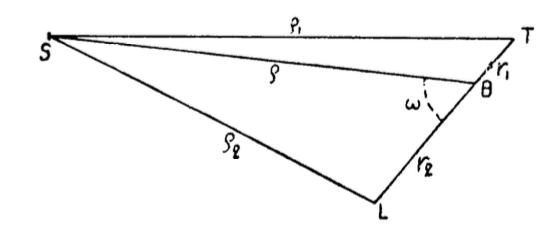
\includegraphics[width=\linewidth]{21}
	\caption{}\label{pic:first}
%	\vspace{5ex}
\end {wrapfigure}
Составим теперь выражения ускорений, которые эти тела сообщают друг другу.
Солнце $S$ сообщает ускорения:
\begin {table}[H]
	\begin {center}
	\vspace{7ex}
		\begin{tabular}{cp{0.09\linewidth}p{0.09\linewidth}p{0.09\linewidth}l}
			Земле: & $\textit{f}\cdot \frac{S}{\rho_1{}^2}$  & \multicolumn{2}{l}{по направлению} & \textit{TS}  \\ [6pt]
			Луне:  & $\textit{f}\cdot \frac{S}{\rho_2{}^2}$  &      $\gg$    &     $\gg$          & \textit{LS}
		\end{tabular}
	\end {center}
\end {table}
вследствие чего точка $\Theta$ имеет ускорения:
\begin {table}[H]
	\begin {center}
		\begin{tabular}{cp{0.09\linewidth}p{0.09\linewidth}p{0.09\linewidth}l}
			$\frac{T}{T+L} \cdot \textit{f} \cdot \frac{S}{\rho_1{}^2}$  & \multicolumn{3}{l}{по направлению, параллельному} & \textit{TS}  \\ [6pt]
			$\frac{T}{T+L}\cdot \textit{f}\cdot \frac{S}{\rho_2{}^2}$  &      $\gg$   &   $\gg$ & $\gg$     & \textit{LS}
		\end{tabular}
	\end {center}
\end {table}


Ускорение Солнца, происходящее от притяжения Земли и Луны, соответственно, суть:
\begin {table}[H]
	\begin {center}
		\begin{tabular}{cp{0.09\linewidth}p{0.09\linewidth}p{0.09\linewidth}l}
			$\textit{f}\cdot \frac{T}{\rho_1{}^2}$  & \multicolumn{2}{l}{по направлению} & \textit{ST}  \\ [6pt]
			$\textit{f}\cdot \frac{L}{\rho_2{}^2}$  &      $\gg$    &     $\gg$          & \textit{SL}
		\end{tabular}
	\end {center}
\end {table}


поэтому ускорения точки $\Theta$ относительно точки \textit{S} будут:

\begin {table}[H]
	\begin {center}
		\begin{tabular}{cp{0.09\linewidth}p{0.09\linewidth}p{0.09\linewidth}l}
			
			$ w _{1} = \textit{f}\cdot \frac{\left(S+T+L\right)}{T+L} \cdot \frac{T}{\rho_1{}^2}$  & \multicolumn{3}{l}{по направлению параллельно} & \textit{TS}  \\ [6pt]
			
			$ w _{2} = \textit{f} \cdot \frac{S+T+L}{T+L} \cdot  \frac{L}{\rho_2{}^2}$  &      $\gg$    & $\gg$ &    $\gg$          & \textit{LS}
			
		\end{tabular}
	\end {center}
\end {table}
Разлагая эти ускорения, соответственно, по направлениям $\Theta$$S$ и $\Theta$$L$, получим, как легко видеть из подобия показанных рис.~\ref{pic:second} и~\ref{pic:third} треугольников:

\begin {table}[H]
	\begin {center}
		\begin{tabular}{cp{0.09\linewidth}p{0.09\linewidth}l}
			$ w _{1}'=  w _{1}\cdot\frac{\rho}{\rho_{1}}$ & \multicolumn{2}{l}{по направлению} & $\Theta$$S$  \\ [6pt]
			
			$ w _{1}''=  w _{1}\cdot\frac{r_{1}}{\rho_{1}}$ &  $\gg$    &  $\gg$ &  $\Theta$$L$  \\ [6pt]
			
			$ w _{2}'=  w _{2}\cdot\frac{\rho}{\rho_{2}}$ &  $\gg$    & $\gg$ &  $\Theta$$S$  \\ [6pt]
		
			$ w _{2}''=  w _{2}\cdot\frac{r_{2}}{\rho_{2}}$ &  $\gg$    & $\gg$ &  $L$$\Theta$
			
		\end{tabular}
	\end {center}
\end {table}

\begin{figure}[H]
	\ffigbox[\FBwidth]{\caption{}\label{pic:second}}
	{ 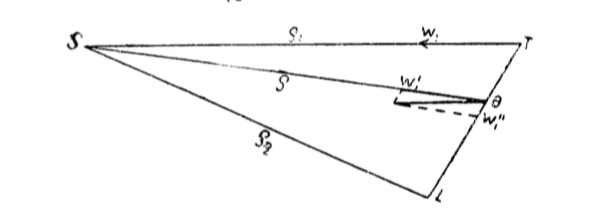
\includegraphics[width=0.9\linewidth]{22} }
	\end {figure}
получим для ускорений точки $\Theta$ слагающие:~

\begin {equation*}
	\begin {aligned}
		W_1 &=  w _{1}' +  w _{2}' = f\cdot\frac{S+T+L}{T+L}\cdot\left[T\cdot\frac{\rho}{\rho_1{}^3}+L\cdot\frac{\rho}{\rho_2{}^3}\right] \mbox{по }\Theta S \\
		W_2 &=  w _{1}'' -  w _{2}'' = f\cdot\frac{S+T+L}{T+L}\cdot\left[T\cdot\frac{r_{1}}{\rho_1{}^3}-L\cdot\frac{r_{2}}{\rho_2{}^3}\right] \mbox{по }\Theta L
	\end {aligned}
\end {equation*}


\begin{figure}[!h]
	\ffigbox[\FBwidth]{\caption{}\label{pic:third}}
	{ 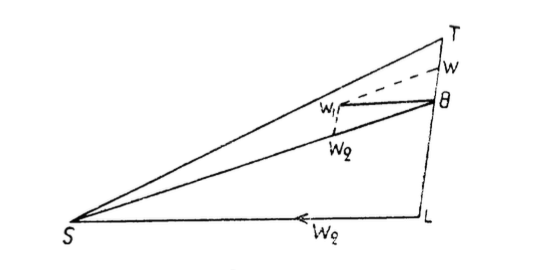
\includegraphics[width=0.8\linewidth]{23} }
\end {figure}


\par{}Заменив $r_1$ и $r_2$ их выражениями~\ref{tab:terms}, имеем:


\begin {align*}
	W_1 &= f\cdot\frac{S+T+L}{T+L}\cdot\rho\cdot\left[\frac{T}{\rho_1{}^3}+\frac{L}{\rho_2{}^3}\right] \mbox{по направлению }\Theta S \\	
	W_2 &=  f\cdot\frac{S+T+L}{\left(T+L\right)^2}\cdot T\cdot L \cdot r \left[\frac{1}{\rho_1{}^3}-\frac{1}{\rho_2{}^3}\right] \mbox{по направлению }\Theta L
\end {align*}

Но
\begin {align*}
	\rho_1{}^2 = \rho^2 + 2\rho\cdot\frac{L}{T+L}\cdot r \cos \omega  + \left(\frac{L}{T+L}\cdot r\right)^2 \\
	\rho_2{}^2 = \rho^2 - 2\rho\cdot\frac{T}{T+L}\cdot r\cos \omega  + \left(\frac{T}{T+L}\cdot r \right)^2
\end {align*}

следовательно:
\begin {align*}
	\frac{1}{\rho_1{}^3} = \frac{1}{\rho^3}\left[1+3\frac{L}{T+L}\cos \omega +\left(\frac{L}{T+L}r\right)^2\left(-\frac32+\frac{15}{2}\cos^2 \omega \right)+\ldots\right]\\
	\frac{1}{\rho_2{}^3} = \frac{1}{\rho^3}\left[1+3\frac{T}{T+L}\cos \omega +\left(\frac{T}{T+L}r\right)^2\left(-\frac32+\frac{15}2\cos^2 \omega \right)+\ldots\right]
\end {align*}
Подставляя эти выражения, имеем:
\begin {align*}
	W_1 &= f\cdot\frac{S+T+L}{\rho^2}\left[1+\frac{T \cdot L}{\left(T+L\right)^2}\cdot\frac{r^2}{\rho^2}\left(-\frac32+\frac{15}2\cos^2 \omega \right)+\ldots\right]\\	
	W_2 &= f\cdot \frac {S+T+L}{\rho^2} \left[-3 \cdot \frac{T\cdot L}{\left(T+L\right)^2}\cdot \frac {r^2}{\rho^2}\cos \omega+\ldots\right]
\end {align*}
Но отношения
\begin {equation*}
	\begin {aligned}
		\frac L{T+L}&\approx\frac1{80}; & \frac r{\rho} &=\frac 1{400}; & \left(\frac r{\rho}\right)^2 &= \frac 1{160000}
	\end {aligned}
\end {equation*}
поэтому будет
\begin {align*}
	\frac{T\cdot L}{\left(T + L\right)^2} \cdot \frac{r^2}{\rho^2}\approx \frac 1{12800000}
\end {align*}
и члены, содержащие этот множитель, могут быть отброшены, так что будет:
\begin {align*}
	W_1 &= f\cdot \frac{S+T+L}{\rho^2} \mbox{ по направлению }\Theta S\\
	W_2 &= 0 \mbox{ по направлению }\Theta L
\end {align*}

Отсюда следут, что точка $\Theta$ движется вокруг Солнца по эллиптический орбите по законам Кеплера.

Рассмотрим теперь ускорение Луны по отношению к Земле, для чего к ускорениям, сообщаемым Луне Солнцем и Землею, надо присовокупить ускорение, равное и противоположное ускорению Земли, происходящему от действия Солнца и Луны. Поступив подобно предыдущему, получим:
	\begin {align*}
		f\cdot\frac{T+L}{r^2}+ f&\cdot S \left[\frac{r_2}{\rho_2{}^3}+\frac{r_1}{\rho_1{}^3}\right]\mbox{ по направлению }L\Theta\\
		f\cdot S \cdot \rho &\left[\frac1{\rho_2{}^3} - \frac1{\rho_1{}^3}\right] \mbox{ параллельно }\Theta S
	\end {align*}
положим:
\begin{alignat*}{4}
	T+L = \mu; & \mbox{  } S = M
\end{alignat*}

\listoftables
\listoffigures




\end{document}

